\addtocontents{toc}{\protect\newpage}
% {Youssouph Cissokho}

\section{Anomalies and large data }\label{Section:4}
%
In this section we refer mainly to [\cite{A1}, \cite{A8}, \cite{A10}, \cite{A14}  \cite{Aurore}].\newl 
The detection of outliers is a broad field that has been studied in a large number of application areas. Nowadays, many real data are very large, in some scenarios the data may contain \textbf{hundreds or thousands of dimensions}. Many recent classical methods use proximity (distance) concepts for anomaly detection and can only be applied in cases where the sample size $n$ is larger than the dimension $p$ ($n>p$). However, the management of large dimensional data i.e. ($n<p$) is another  critical issue. Indeed, in a space data points become isolated and scattered and the notion of proximity fails to maintain its importance. Consequently, the notion of defining significant outliers is much more complex and not obvious.  Thus, many conventional methods of detecting outliers do not work effectively, \textbf{this is an artifact known as the curse of dimensionality}.\newl
The remainder of this section is organized as follows: first, an attempt is made to define the concept and the challenges, then the techniques for detecting outliers are discussed and finally, \textbf{ensemble and subspace} methods will be presented in details. 
%
%
\subsection{Definitions and Challenges}
%
%
An outlier is an observation that deviates or behaves differently from other observations in the data that gives rise to suspicion that it was generated by another mechanism. An outlier is also referred to as an abnormality, discrepancy, anomaly, or deviation in the data mining and statistical literature \cite{A1}.
The challenges in detecting large dimensional outliers or anomalies lie in the fact that,
\begin{itemize}
\item The notion of distance fails to retain its importance due to the curse of dimensionality. Hence << the problem of detecting outliers is like finding a needle in a haystack >> \cite{A14};
\item Every point tends to become an outlier;
\item The dataset becomes more sparse as number of dimensions increase.
\end{itemize}

\noindent The authors of \cite{AYU} consider that in order to deal properly with large datasets, detection methods should have the characteristics of following:
\begin{enumerate}[noitemsep]
\item Effective management of sparse data issues.
\item Interpretability of the discrepancy, i.e. why this observation behaved differently.
\item Comparability of the measure of abnormality.
\item Consideration of local data behaviour to determine whether an observation is abnormal or not.
\end{enumerate}
%
\subsection{Method based on projection into subspaces: ACP, DOBIN}
%
Nowadays, it is common to have very large data sets known as HDLSS (High dimension low sample size), which can contain hundreds of dimensions, and as a result, conventional methods of detecting anomalies or outliers do not work very effectively. One of the solutions to this problem is to reduce the dimension, while keeping the essential characteristics of the data. This is called dimensionality reduction. Examples include, but are not limited to, \textbf{ principal component analysis, linear discriminant analysis, feature selection, etc}. Two classical approaches are \textbf{characteristic selection}, which consists in selecting a small set of variables representative of the observations, and \textbf{principal component analysis}, which will be the subject of a detailed study in the following.
%
\subsubsection*{Principal Component Analysis (PCA)}
%
Principal Component Analysis (PCA) aims to find a representation in the lower dimensional space (projecting points on a line, a plane, ... a subspace) of the data containing the greatest possible variation. It therefore corresponds to an orthogonal linear transformation transforming the data into a new coordinate system, so that the largest variance resulting from a scalar projection of the data is on the first coordinate (called the first principal component), the second largest variance on the second coordinate, etc. The PCA is a linear transformation of the data into a new coordinate system. It can therefore be used for two purposes:
\begin{itemize}
    \item Dimension reduction could be used as a pre-processing step;
    \item It could also be used as a detector of outlierness.
    \item Furthermore, it also allows a lower dimensional visualization (2 or 3 dimensions), which could not be done in a greater dimension.
\end{itemize}

Given a matrix of the $n\times p$ data, $\textbf{X}=(X_1,\cdots,X_p)$ of $n$ observations (number of rows) and $p$ variables (number of columns) centered and reduced. The main components, which are a linear combination of the variables, are given by the following variables,
\begin{align*}
\textbf{Y}_i=\ell^t_i\textbf{X}=\ell_{1i}\textbf{X},\cdots,\ell_{pi}\textbf{X};\quad i=1,\cdots,k.
\end{align*}
with ($k\leq p$), which provides the largest variance subject to the $\|\ell_i\|=1$ constraint (where $\|\cdot\|$ is the norm). 
Therefore,
\begin{align*}
\operatorname{var}\left(Y_{i}\right) &=\operatorname{var}\left(\ell_{i}^{t} \boldsymbol{X}\right)=\ell_{i}^{t} \boldsymbol{\Sigma} \ell_{i} \,,\\ 
\operatorname{cov}\left(Y_{i}, Y_{k}\right) &=\operatorname{cov}\left(\ell_{i}^{t} \boldsymbol{X}, \ell_{k}^{t} \boldsymbol{X}\right)=\ell_{i}^{t} \boldsymbol{\Sigma} \ell_{k}\, .
\end{align*}
In other words 
find the vector $\ell_{i}$ that maximizes the variance of $Y_i$ i.e.
\begin{align*}
\mathbf{\ell}_{1}&=\underset{\|\mathbf{\ell_1}\|=1}{\arg \max }\left\{\ell^t_1\mathbf{X}^{t} \mathbf{X} \ell_1\right\},
\end{align*}
and $\ell_2$ such that the variance is maximal and uncorrelated with $\ell_1$,   
\begin{align*}
\mathbf{\ell}_{2}& =\underset{\|\mathbf{\ell_2}\|=1,\;\ell_{1}^{t}\ell_{2} =0}{\arg \max }\left\{\ell^t_2\mathbf{X}^{t} \mathbf{X} \ell_2\right\}.
\end{align*}
Similarly, we find $\ell_k$ such that the variance is maximal and uncorrelated with all the $\ell_i$, $i<k$ i.e.
\begin{align}
\mathbf{\ell}_k=\underset{\substack{\|\ell_k\|=1,\\ \;\ell_{i}^{t}\ell_k=0,\;\forall\;i<k}}{\arg \max} \left\{\ell^t_k\mathbf{X}^t \mathbf{X} \ell_k\right\}.\label{eq1}
\end{align}
To solve \eqref{eq1}, for all $\;i<k$, we use the Lagrangian which is given by 
\begin{align*}
L=\ell^t_k\mathbf{X}^t \mathbf{X} \ell_k-\lambda_k(\ell^t_k\ell_k-1)-w\ell_{i}^{t}\ell_k.
\end{align*}
Deriving the Lagrangian with respect to each of the components of the vector $\ell_k$, $\lambda_k$ et $w$ simplifiant, on trouve: 
\begin{align}
\mathbf{X}^t \mathbf{X} \ell_k&=\lambda_k\ell_k\\
\ell^t_k\ell_k&=1,\; \text{and}\; \ell^t_k\ell_i=0,\;\text{for all}\; i<k.
\end{align}
The $\ell_k$ vector corresponds to the eigenvector associated with the $k$th largest eigenvalue of the $\mathbf{X}^t \mathbf{X}$ matrix. Hence the following result:
\begin{lemma}
The $k$ ($k<p$) principal components giving the largest maximum variance are given by the $k$ eigenvectors associated with the $k$ largest eigenvalues of $\mathbf{X}^t \mathbf{X}$.
\end{lemma}
\textbf{Proportion of variance explained}, we note that 
\begin{align*}
\sum_{i=1}^{k}\operatorname{var}\left(Y_{i}\right) &=\sum_{i=1}^{k}\ell_{i}^{t} \boldsymbol{\Sigma} \ell_{i}=\sum_{i=1}^{k}\lambda_i \,.
\end{align*}
Thus, the total variance of the population is equal to the sum of the eigenvalues. Therefore, the proportion of the total variance explained by the i-th main component is 
\begin{align*}
0\leq \frac{\lambda_i}{\sum_{i=1}^{p}\lambda_i }\leq 1
\end{align*}
\textbf{How many components to retain?}, 
The quality of the CPA results is highly dependent on the number of major components selected, i.e. the $k$ dimension of the subspace. There are several methods that address this problem, just two of which are presented here: \textbf{the share of total variance explained by the $k$ first principal component} and \textbf{the scree method}.
\textbf{The total variance explained by the $k$ first principal axes}, is given by 
\begin{align*}
p_k=\frac{\sum_{i=1}^{k} \lambda_i}{\sum_{i=1}^{p}\lambda_i }
\end{align*}
We thus retain the $k$ main components so that $p_k$ is higher than a predefined value (often it is between $80\%$ and $90\%$). \newl
\textbf{the Scree method}, consists of plotting the eigenvalue curve in a decreasing manner. The principle consists in locating, if there is a "bend" in the graph and keeping only the eigenvalues up to this bend.
\begin{example}
An example applied to \href{1http://web.stanford.edu/ hastie/CASIles/DATA/leukemia big.csv}{data} measurements of gene expression in 72 patients with leukemia. It consists of $7128$ genes. See Figure \ref{fig0}.
\begin{figure*}[t]
    \centering
     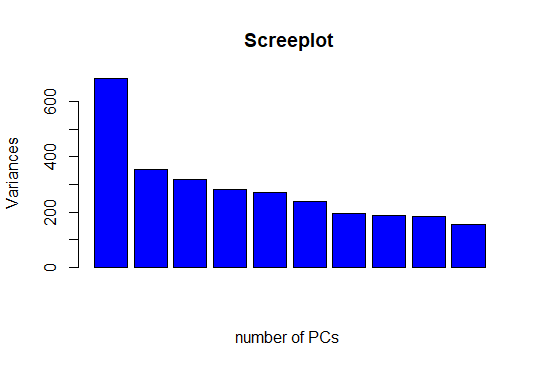
\includegraphics[width=.5\textwidth]{\MainFolder/Images/screeleuk.png}
    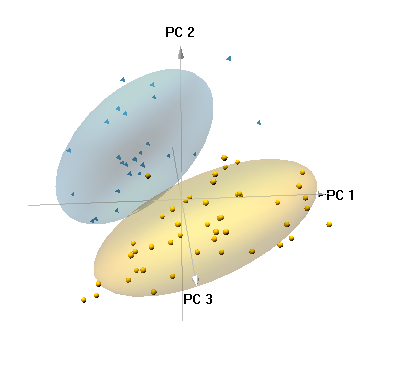
\includegraphics[width=.4\textwidth]{\MainFolder/Images/3dpcleuk.PNG}
    \caption{Screeplot (left), 3-component data projection (right)}\hrule
    \label{fig0}
\end{figure*}
\end{example}
\noindent There are other methods of reducing dimensionality such as SVD (Singular Value Decomposition).
%
%
\subsubsection*{A Distance based Outlier BasIs using Neighbours (DOBIN)}
 DOBIN has two main uses. Firstly, as a more favourable basis for detecting outliers, it brings distant values to the forefront by using a reduced number of components. In this sense, it is somewhat similar to the detection of outliers in subspace, although DOBIN does not directly detect outliers. If outliers appear in the full input space, DOBIN allows the outlier detection algorithm to detect the outliers using fewer components. \cite{A7}.  
 
 Let $X_{N\times p}$ be a matrix of data with $N$ observations and $p$ dimensions. One notes the i-th row of $X$ by $x_i$, the distance between $x_i$ and $x_j$ can be written as follows
 \begin{align*}
 d(x_i,x_j)^2=(x_i-x_j)^tS(x_i-x_j) 
 \end{align*}
 where $S$ is a symmetric and positive definite matrix. If $S=diag(s_1,\cdots,s_p)$ is a diagonal matrix, then
 \begin{align}\label{dob1}
 d(x_i,x_j)^2=\langle\eta,(x_i-x_j)\circ(x_i-x_j) \rangle
 \end{align} 
 where $\langle\cdot{,}\cdot\rangle$ denotes the standard inner product in $R^p$, $\eta = (s_1,\cdot,s_p)$ and $\circ$ denotes the product per element. Since $S$ is a symmetric and positive definite, it is diagonalizable, which motivates to consider a diagonal $S$. The key element of DOBIN lies in the construction of the $Y$ space.
 Let $y_{ij}=(x_i-x_j)\circ(x_i-x_j)$, therefore \eqref{dob1} becomes 
\begin{align}\label{dob2}
d(x_i,x_j)^2=\langle\eta,y_{ij}\rangle.
\end{align}

 The goal now is to find a unit vector $\eta$ that will maximize the distance between $x_i$ and $x_j$. Calculating $y_{ij}$ for all pairs would be expensive because there are $N (N + 1) / 2$ pairs to consider. Moreover, it would give us pairwise distances between points that we are not interested in, such as points at the edge of the point cloud. Finding $\eta$ that maximizes the distances between such points is not beneficial for outlier detection, because a large distance between opposing points does not mean that any of them are outliers \cite{A7}. The following algorithm summarizes the calculation of the $Y$ space.
\begin{algorithm}
\SetAlgoLined
$X_1$=norm1($X$)\;
Look for $k1$ to $k2$ neighbors of each point in $X_1$\;
$X_2$=norm2($X$)\;
Look for $k1$ to $k2$ next to each point in $X_2$\;
Then, for each point, collect all the unique neighbors obtained in steps 2 and 3;
Set $T=\{(i,j): \quad i,j\in X\}$\;
For all these pairs, compute $y_{ij}$ as in the equation \eqref{dob2} using $X_1$ or $X_2$\;

Let $Y=\{y_1=y_{i_1j_1},\cdots,y_m=y_{i_mj_m}\}$
with $y_{i_kj_k}$ the kth pair in T, so $Y$ is a $m \times p$\ matrix with $y_\ell$ the $\ell$th line\;

Let $Q$ be the $q$th percentile of $d=\sum_k^p y_{\ell k}$ with $d$ the distance between $x_{i_\ell}$ and $
x_{j_\ell}$ in $X_1$ or $X_2$.\;
Remove the points where $d<Q$ and the corresponding pairs $(i,j)$ in T.\;
The remaining points are the space $Y=\{y_\ell \}^M_{\ell=1}$\;
\KwResult{ The $Y$ space consisting of $\{y_\ell \}^M_{\ell=1}$ and the corresponding $i$ and $j$ indices }
\caption{Construction of space $Y$: Data $X$, $k1$, $k2 \in Z^+$, $q\in (0, 1)$ and the choice of normalization.}
\end{algorithm}\newl
\textbf{Maximize distance between points:}
rewriting equation \eqref{dob2} using $T(\ell)=(i,j)$
\begin{align}\label{dob3}
\sum_{(i,j)\in T}d(x_i,x_j)^2=\sum_\ell \langle\eta,y_\ell\rangle.
\end{align}
The  unit vector $\eta$ that maximizes this equation is $$\displaystyle \eta=\frac{\sum_\ell^M y_\ell}{\|\sum_\ell^M y_\ell\|},$$ where $M$ is obtained in algorithm 1.\newl
\textbf{Construction of a basis of $Y$: }
A basis is constructed via the following relationship,
\begin{align*}
y_{\ell_b}=y_{\ell_{b-1}}- \langle\eta_b,y_{\ell_{b-1}}\rangle \eta_b\qquad\text{et}\quad
\eta_{b+1}=\frac{\sum_\ell^M y_{\ell_b}}{\|\sum_\ell^M y_{\ell_b}\|}
\end{align*}
where $y_{\ell_0}=y_\ell$. The set $\Theta=(\eta_1,\cdots,\eta_p)$ constitutes a basis of $Y$.  With this basis, the final result is obtained by 
\begin{align}\label{newx}
\Tilde{X}=X_1\Theta \qquad\text{ou}\quad \tilde{X}=X_2\Theta.
\end{align}
This basis is invariant by addition but not to rotations. In summary, 
 the objective of DOBIN is to:
 \begin{itemize}
 \item Find the $Y$ space for a given $X$ dataset, as shown in Algorithm 1.
 \item Build the basis as shown above.
 \item Transform the original $X$ space using the equation \eqref{newx}. 
 \end{itemize}
 Figure \ref{fig00} shows the two spaces $X$ and $Y$ where $X$ is a normal distribution 
 of $100$  points with a single outlier shown in red. The $Y$ space consists of fewer points than the $X$ space, with $6$ points coming from the outlier. Indeed, in the construction of the $Y$ space, $5$ neighbors are considered for each point with $k1 =1$ to $k2 = 5$.
 \begin{figure*}[ht]
    \centering
     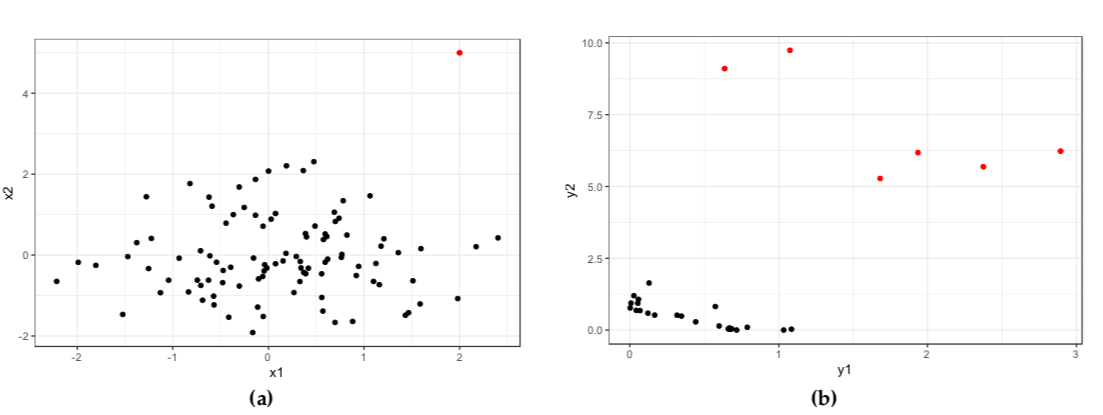
\includegraphics[width=\textwidth]{\MainFolder/Images/ysapce.png}
    \caption{The $X$ and $Y$ spaces. The $X$ space in (a) and the associated $Y$ space in (b) with $q = 0.95$. The dot colored red in the $X$ space gives rise to 6 dots, which are colored red in the $Y$ space (source \cite{A6}).}\hrule
    \label{fig00}
\end{figure*}

%
\subsection{Ensembles method}
%
%
In the previous sections, various anomaly detection algorithms have been described, the relative performance of which varies with the type of data being considered. It is often impossible to find one algorithm that outperforms all others. This is because a particular anomaly detection algorithm \textbf{may be well suited to a particular data set and be successful in detecting abnormal or outlier} observations, but may not work with other data sets whose characteristics do not match the first data set. The impact of such a mismatch between algorithms can be mitigated by using a \textbf{set of algorithms} where the results of several algorithms are considered before making a final decision, these methods often provide the best results and thus improve the performance of the other methods \cite{A10}. There are two types of ensemble methods: \textbf{sequential ensemble  and independent ensemble}, \newl
\subsection*{Sequential ensembles}
In sequential ensembles, a given algorithm or a set of algorithms are applied sequentially, so that future applications of the algorithms can be applied sequentially reuse previously obtained results and so on. The final result is either a weighted combination of all the results or the final result of the last application of the last algorithm. 

\begin{algorithm}
\SetAlgoLined
j=1\;
\While{As long as the condition is verified }{
	Take an algorithm $A_j$ based on the results of the
	previous executions\;
	Create a new $f_j(D)$ of data D based on the results of the
	previous executions\;
	Apply $A_J$ to $D_J$\;
	d=j+1\;
}
\KwResult{Returning outliers based on the combination of results from previous runs  }
\caption{SequentialEnsembles(Data: D,
	Base algorithms: $A_1,\cdots,A_r$)}
\end{algorithm}%\newl
\subsection*{Independent ensembles}
In sequential ensembles, different algorithms, or different instantiations of the same algorithm are applied either to the complete dataset or parts of it. Choices made about the dataset 
and the algorithms applied are independent of the results obtained. from the various executions. The results are combined to obtain more robust outliers.

\begin{algorithm}
\SetAlgoLined
j=1\;
\While{As long as the condition is verified }{
	Take an algorithm $A_j$\;
	Create a new data $f_j(D)$ from data D\;
	Apply $A_j$ to $f_j(D)$\;
	j=j+1\;
}
\KwResult{Returning outliers based on the combination of results
	of previous executions  }
\caption{IndependentEnsembles(Data: D,
	Base algorithms: $A_1,\cdots,A_r$)}
\end{algorithm}
In this method, each algorithm provides an anomaly result.
objects in $D$; objects that receive higher scores are considered more abnormal. To combine or aggregate the results to obtain more robust outliers or anomalies, several techniques are used: \textbf{majority vote, mean, min-rank method}. For example, to combine or aggregate the results to obtain more robust outliers or anomalies, several techniques are used: \textbf{majority voting, mean, min-rank method}, 
we note $\alpha_i(p)$, is the normalized anomaly score of $p\in D$, according to algorithm $i$. A value close to $0$ indicates a weak anomaly, and a value equal to $1$ indicates a strong anomaly. We note by $r_i(p)$ the rank of $p\in D$, the first rank is assigned to the element with a strong anomaly, and 2 to the element with a weaker anomaly, and so on. If $m$ algorithms are considered, then
\begin{align}
\alpha(p)=\frac{1}{m}\sum_{i=1}^{m}\alpha_i(p) \qquad \text{et}\; \qquad r(p) =\min_{1\leq i \leq m} r_i(p).
\end{align}
 Three-point data is considered, after the application of three
algorithms $A_1, A_2$ and $A_3$, we have 
\begin{align*}
	\alpha_{1}\left(p_{1}\right)&=1.0,\; \alpha_{1}\left(p_{2}\right)=0.9,\; \alpha_{1}\left(p_{3}\right)=0.0; \\ 
\alpha_{2}\left(p_{1}\right)&=1.0,\; \alpha_{2}\left(p_{2}\right)=0.8,\; \alpha_{2}\left(p_{3}\right)=0.0;\\
\alpha_{3}\left(p_{1}\right)&=0.1,\;  \alpha_{3}\left(p_{2}\right)=1.0,\; \alpha_{3}\left(p_{3}\right)=0.0.
\end{align*}
The averaging method gives 
\begin{align*}
\alpha\left(p_{1}\right)&=.7,\; \alpha\left(p_{2}\right)=0.9,\; \alpha\left(p_{3}\right)=0.0,
\end{align*}
indicating that $p_2$ is more abnormal than $p_1$. For the minimum rand method,
\begin{align*}
r_{1}\left(p_{1}\right)&=1,\; r_{1}\left(p_{2}\right)=2,\; r_{1}\left(p_{3}\right)=3;\\ 
r_{2}\left(p_{1}\right)&=1,\; r_{2}\left(p_{2}\right)=2,\; r_{2}\left(p_{3}\right)=3;\\
r_{3}\left(p_{1}\right)&=2,\; r_{3}\left(p_{2}\right)=1,\; r_{3}\left(p_{3}\right)=3.
\end{align*}
In this case, the minimum rank obtained is
\begin{align*}
r\left(p_{1}\right)=1,\; r\left(p_{2}\right)=1,\; r \left(p_{3}\right)=3.
\end{align*}
$p_1$ and $p_2$ have the same degree of anomaly, but more abnormal than $p_3$. 
Which combination function provides the best information for the overall analysis? Clearly, the combination function may depend on the structure of the dataset. However, in the general case, the two most commonly used functions are the maximum and average method.
%
\subsection{Sub-space method}
%
%
Ensemble analysis has been used particularly effectively in the detection of large outliers [\cite{A8}, \cite{A13}, \cite{A14}], in which several subspaces of the data are often searched for outliers, as they are often hidden in \textbf{smaller subspaces}. It is therefore logical to explore the \textbf{lower dimensional subspaces} [\cite{A1}, \cite{A2}]. Such an approach eliminates the additive noise effects of many dimensions and leads to more robust outliers. Such a problem is very difficult to solve effectively. This is due to the fact that the number of possible projections of large dimensional data is exponentially related to the dimensionality of the data. The problem of outlier detection is like finding a needle in a haystack \cite{A14}.
Feature bagging algorithm is presented below
\begin{algorithm}
\SetAlgoLined
j=1\;
\While{As long as the condition is verified }{
  Randomly draw an integer $r$ such that $d/2\leq r\leq d- 1$\;
	Select $r$ dimensions ( variables) from the data randomly to create a $r$ dimension projection\;
	Find LOF score for each point in the projected representation\;
	j=j+1\;
}
\KwResult{Report combined score based on different subspaces}
\caption{FeatureBagging(Data: D)}
\end{algorithm}

\noindent There are many different algorithms in the literature, including the \textbf{HOS} (High-dimensional Outlying Subspaces) \cite{Zhang}; \textbf{SOD} (Subspace Outlier Degree) \cite{Zi} implemented in the \textbf{HighDimOut} package; \textbf{OutRank} (Projected Clustering Ensembles) \cite{M1}; \textbf{OUTRES} (Local Selection of Subspace Projections) \cite{M3}.

In summary, it should be noted that anomaly detection and outlier analysis is still an open field with many challenges. There is no magic method, all methods have strengths. 
\afterpage{\FloatBarrier}